\documentclass[aspectratio=169,10pt]{beamer}
\newcommand{\TalkShort}{EconophysicsLab offsite 2026}
% Visual reference: Matteo Di Sante, 13_06_26_slides_soaring_ctrw.tex.
% Steel-blue title bar, Palatino, Pisa seal, white pages and a pale title band.
\usepackage[T1]{fontenc}
\usepackage[utf8]{inputenc}
\usepackage[english]{babel}
\usepackage{mathpazo}
\usefonttheme{serif}
\usepackage{amsmath,amssymb,bm,booktabs,array,graphicx,tikz,microtype}
\usetikzlibrary{arrows.meta,calc,positioning}
\usepackage{siunitx}
\sisetup{group-separator={,},group-minimum-digits=4}
\usepackage{pgfpages}
\ifdefined\Speakernotes
  \setbeameroption{show notes on second screen=right}
\else
  \setbeameroption{hide notes}
\fi
\definecolor{pisablue}{RGB}{74,96,121}
\definecolor{pisablight}{RGB}{192,206,220}
\definecolor{accent}{RGB}{26,118,179}
\definecolor{para}{HTML}{3477A8}
\definecolor{hang}{HTML}{B5482A}
\definecolor{beginner}{HTML}{6A3D9A}
\definecolor{expert}{HTML}{C98A1E}
\definecolor{teal}{HTML}{2E7D8A}
\definecolor{wine}{HTML}{8E3B5C}
\definecolor{muted}{HTML}{666666}
\setbeamercolor{structure}{fg=pisablue}
\setbeamercolor{normal text}{fg=black,bg=white}
\setbeamercolor{frametitle}{fg=white,bg=pisablue}
\setbeamercolor{alerted text}{fg=accent}
\setbeamercolor{block title}{fg=white,bg=pisablue}
\setbeamercolor{block body}{fg=black,bg=pisablight!28}
\setbeamercolor{discussion}{fg=pisablue,bg=pisablight!30}
\setbeamercolor{button}{fg=white,bg=pisablue}
\setbeamerfont{button}{size=\normalsize}
\setbeamersize{text margin left=7mm,text margin right=7mm}
\setbeamertemplate{navigation symbols}{}
\setbeamertemplate{itemize item}{\textcolor{pisablue}{\small$\bullet$}}
\setbeamertemplate{itemize subitem}{\textcolor{pisablue}{\textendash}}
\setbeamertemplate{itemize/enumerate body begin}{\setlength{\itemsep}{0.55em}}
\setbeamertemplate{frametitle}{%
  \nointerlineskip
  \begin{beamercolorbox}[wd=\paperwidth,ht=9mm,dp=3mm,center]{frametitle}
    \large\insertframetitle\strut
  \end{beamercolorbox}
  \begin{tikzpicture}[remember picture,overlay]
    \node[anchor=north west,inner sep=0pt,xshift=2mm,yshift=-1.2mm]
      at(current page.north west){
\includegraphics[height=8mm]{assets/cherubino_white.png}};
    \node[anchor=north east,text=white,inner sep=0pt,xshift=-2.3mm,yshift=-4.2mm]
      at(current page.north east){\small\insertframenumber};
  \end{tikzpicture}
}
\setbeamertemplate{footline}{%
  \hspace{7mm}\textcolor{muted}{\fontsize{6.5}{8}\selectfont
    Matteo Di Sante\enspace|\enspace\TalkShort\enspace|\enspace13 September 2026}
  \hfill\textcolor{muted}{\fontsize{6.5}{8}\selectfont Supervisor discussion}\hspace{7mm}\vspace{2mm}
}
\newcommand{\kw}[1]{\textcolor{accent}{#1}}
\newcommand{\source}[1]{\par\vspace{1mm}{\fontsize{7}{8.3}\selectfont\color{muted}#1\par}}
\newcommand{\question}[1]{\par\vfill
  \begin{beamercolorbox}[wd=\linewidth,sep=5pt]{discussion}
    \small #1
  \end{beamercolorbox}}
\newcommand{\fig}[2][54mm]{\includegraphics[width=\linewidth,height=#1,keepaspectratio]{assets/#2}\par}
\newcommand{\speaker}[1]{\note{#1}}
\setbeamertemplate{note page}{%
  \vspace{4mm}\noindent%
  \begin{minipage}{\linewidth}
    {\small\color{pisablue}\TalkShort\quad|\quad Slide \insertframenumber}\par\medskip
    {\normalsize\bfseries\insertframetitle}\par\medskip
    {\small\insertnote}
  \end{minipage}
}
\newcommand{\refitem}[3]{\href{#1}{#2}\hfill {\color{muted}#3}\par\medskip}
\newcommand{\titleframe}[4]{%
\begin{frame}[plain]
\begin{tikzpicture}[remember picture,overlay]
 \fill[pisablue](current page.south west)rectangle(current page.north east);
 \fill[pisablight](current page.south west)rectangle([yshift=20mm]current page.south east);
 \node[anchor=north,yshift=-4mm]at(current page.north){
\includegraphics[height=13mm]{assets/cherubino_white.png}};
 \node[text=white,align=center]at([yshift=19mm]current page.center)
   {{\scshape\large University of Pisa}\\[2mm]{\small Department of Physics ``Enrico Fermi''}};
 \node[text=white,align=center,text width=.92\paperwidth]at([yshift=-3mm]current page.center)
   {{\LARGE\bfseries #1}\\[3mm]{\large #2}};
 \node[text=pisablue,align=center]at([yshift=10mm]current page.south)
   {{\normalsize Matteo Di Sante}\quad$\bullet$\quad{\normalsize 13 September 2026}\\[2mm]
    {\small #3}};
\end{tikzpicture}
\note{#4}
\end{frame}}
\newcommand{\backupstart}{%
\appendix
\begin{frame}[plain,noframenumbering]
\begin{tikzpicture}[remember picture,overlay]
 \fill[pisablue](current page.south west)rectangle(current page.north east);
 \node[text=white,align=center]at(current page.center)
  {{\LARGE\bfseries Discussion material}\\[4mm]{\large Extra figures, derivations and references}};
\end{tikzpicture}
\end{frame}}
\hypersetup{colorlinks=true,urlcolor=accent,linkcolor=accent,pdfauthor={Matteo Di Sante}}
% A notes sheet contains a second rendering of the slide. Disable its duplicate
% destinations; the normal slide PDF retains all hyperlinks and the viewer button.
\ifdefined\Speakernotes\hypersetup{draft}\fi

% AUTO-GENERATED by scripts/reporting/generate_stats.py -- DO NOT EDIT.
\newcommand{\StatGenerated}{2026-07-24}
\newcommand{\StatParaNumSeasons}{27}
\newcommand{\StatParaSeasonFirst}{1999--2000}
\newcommand{\StatParaSeasonLast}{2025--2026}
\newcommand{\StatParaTotalFlights}{203343}
\newcommand{\StatParaWithIgc}{186225}
\newcommand{\StatParaDownloaded}{186052}
\newcommand{\StatParaPctWithIgc}{91.6}
\newcommand{\StatParaPctDownloaded}{99.9}
\newcommand{\StatHangNumSeasons}{25}
\newcommand{\StatHangSeasonFirst}{2001--2002}
\newcommand{\StatHangSeasonLast}{2025--2026}
\newcommand{\StatHangTotalFlights}{9259}
\newcommand{\StatHangWithIgc}{6746}
\newcommand{\StatHangDownloaded}{6716}
\newcommand{\StatHangPctWithIgc}{72.9}
\newcommand{\StatHangPctDownloaded}{99.6}
\newcommand{\StatTotalFlights}{212602}
\newcommand{\StatTotalWithIgc}{192971}
\newcommand{\StatTotalDownloaded}{192768}

% Generated by scripts/reporting/ch2_dataset/generate_pipeline_census.py -- do not edit.
\newcommand{\StatPipeParaAttempted}{186052}
\newcommand{\StatPipeParaKept}{156449}
\newcommand{\StatPipeParaKeptPct}{84.1}
\newcommand{\StatPipeParaBaroWitnessPct}{72.1}
\newcommand{\StatPipeParaDropPipelineRaised}{0}
\newcommand{\StatPipeParaDropFewerThanTwoFixes}{27}
\newcommand{\StatPipeParaDropNoUsableAltitudeChannel}{697}
\newcommand{\StatPipeParaDropNoSustainedFlight}{197}
\newcommand{\StatPipeParaDropCleaningRebuiltTooMuch}{374}
\newcommand{\StatPipeParaDropDurationBelowMinimum}{2090}
\newcommand{\StatPipeParaDropDurationAboveMaximum}{3}
\newcommand{\StatPipeParaDropPathBelowMinimum}{174}
\newcommand{\StatPipeParaDropAltitudeRangeBelowMinimum}{4900}
\newcommand{\StatPipeParaDropMeanGroundSpeedAboveTheFixLevelBound}{0}
\newcommand{\StatPipeParaDropExtentOutOfReachOfTheFirstFix}{217}
\newcommand{\StatPipeParaDropNoNativeCadence}{0}
\newcommand{\StatPipeParaDropNoSegmentSurvived}{20923}
\newcommand{\StatPipeParaDropShorterThanSmoothingWindow}{1}
\newcommand{\StatPipeParaMedianDurationMin}{158}
\newcommand{\StatPipeParaMedianPathKm}{89}
\newcommand{\StatPipeParaMedianDtS}{1}
\newcommand{\StatPipeParaSplitPct}{6.8}
\newcommand{\StatPipeParaMedianSegments}{1}
\newcommand{\StatPipeParaInterpPct}{0.58}
\newcommand{\StatPipeParaTrimmedPct}{1.32}
\newcommand{\StatPipeParaRemovedPct}{1.83}
\newcommand{\StatPipeParaAltInvalidPct}{0.015}
\newcommand{\StatPipeParaFlaggedKeptPct}{0.68}
\newcommand{\StatPipeParaFrozenFlightsPct}{31.3}
\newcommand{\StatPipeParaBoundariedFlightsPct}{0.12}
\newcommand{\StatPipeParaBoundariedTotal}{1700}
\newcommand{\StatPipeParaInSegmentSteps}{1371359594}
\newcommand{\StatPipeHangAttempted}{6716}
\newcommand{\StatPipeHangKept}{6102}
\newcommand{\StatPipeHangKeptPct}{90.9}
\newcommand{\StatPipeHangBaroWitnessPct}{84.6}
\newcommand{\StatPipeHangDropPipelineRaised}{0}
\newcommand{\StatPipeHangDropFewerThanTwoFixes}{0}
\newcommand{\StatPipeHangDropNoUsableAltitudeChannel}{135}
\newcommand{\StatPipeHangDropNoSustainedFlight}{1}
\newcommand{\StatPipeHangDropCleaningRebuiltTooMuch}{40}
\newcommand{\StatPipeHangDropDurationBelowMinimum}{83}
\newcommand{\StatPipeHangDropDurationAboveMaximum}{0}
\newcommand{\StatPipeHangDropPathBelowMinimum}{1}
\newcommand{\StatPipeHangDropAltitudeRangeBelowMinimum}{155}
\newcommand{\StatPipeHangDropMeanGroundSpeedAboveTheFixLevelBound}{0}
\newcommand{\StatPipeHangDropExtentOutOfReachOfTheFirstFix}{5}
\newcommand{\StatPipeHangDropNoNativeCadence}{0}
\newcommand{\StatPipeHangDropNoSegmentSurvived}{194}
\newcommand{\StatPipeHangDropShorterThanSmoothingWindow}{0}
\newcommand{\StatPipeHangMedianDurationMin}{184}
\newcommand{\StatPipeHangMedianPathKm}{163}
\newcommand{\StatPipeHangMedianDtS}{3}
\newcommand{\StatPipeHangSplitPct}{16.2}
\newcommand{\StatPipeHangMedianSegments}{1}
\newcommand{\StatPipeHangInterpPct}{0.31}
\newcommand{\StatPipeHangTrimmedPct}{0.84}
\newcommand{\StatPipeHangRemovedPct}{0.72}
\newcommand{\StatPipeHangAltInvalidPct}{0.006}
\newcommand{\StatPipeHangFlaggedKeptPct}{0.96}
\newcommand{\StatPipeHangFrozenFlightsPct}{65.4}
\newcommand{\StatPipeHangBoundariedFlightsPct}{0.36}
\newcommand{\StatPipeHangBoundariedTotal}{3055}
\newcommand{\StatPipeHangInSegmentSteps}{34583916}
\newcommand{\PipeCensusTable}{%
\begin{tabular}{|l|r|r|}
\hline
\textbf{Why the flight was dropped} & paragliders & hang gliders \\
\hline
unreadable track & 27 & 0 \\
no usable GNSS altitude & 697 & 135 \\
never airborne & 197 & 1 \\
integrity gate & 374 & 40 \\
shorter than the duration cut & 2{,}090 & 83 \\
longer than the duration cut & 3 & 0 \\
path below the floor & 174 & 1 \\
altitude activity below the floor & 4{,}900 & 155 \\
out of reach of its own first fix & 217 & 5 \\
no segment survived resampling & 20{,}923 & 194 \\
no segment carries the smoothing window & 1 & 0 \\
\hline
\textbf{retained} & \textbf{156{,}449} (84.1\%) & \textbf{6{,}102} (90.9\%) \\
\hline
\end{tabular}}

% Generated by scripts/tesi/ch03_fixed_transport/write_ch3_text.py
% Chapter prose is hand-written; only these values are generated.
\newcommand{\ChThreeClosedAltShiftMax}{0.051}
\newcommand{\ChThreeClosedAltShiftMin}{0.021}
\newcommand{\ChThreeCohortBiasMaxPct}{2.0}
\newcommand{\ChThreeCohortBiasMinPct}{1.8}
\newcommand{\ChThreeCohortShiftMax}{0.0177}
\newcommand{\ChThreeCohortShiftMin}{0.0164}
\newcommand{\ChThreeEligibleClosed}{87,807}
\newcommand{\ChThreeEligibleClosedPct}{56.6}
\newcommand{\ChThreeEligibleOpen}{67,003}
\newcommand{\ChThreeEligibleOpenPct}{43.2}
\newcommand{\ChThreeEligibleUnknown}{275}
\newcommand{\ChThreeGeneralFitLagMax}{30000}
\newcommand{\ChThreeGeneralFitLagMin}{10}
\newcommand{\ChThreeGeneralLastFitLag}{28440}
\newcommand{\ChThreeHangClosedFracMain}{76.5}
\newcommand{\ChThreeHangClosedFracStart}{64.0}
\newcommand{\ChThreeHangCohortOverlapPct}{99.7}
\newcommand{\ChThreeHangGeneralGroups}{7}
\newcommand{\ChThreeHangGeneralHurst}{0.841 [0.816, 0.855]}
\newcommand{\ChThreeHangGeneralReplicates}{998}
\newcommand{\ChThreeHangGeneralRms}{0.075}
\newcommand{\ChThreeHangGeneralRmsRatio}{1.19}
\newcommand{\ChThreeHangKurtEEnd}{4.03}
\newcommand{\ChThreeHangKurtEStart}{-0.60}
\newcommand{\ChThreeHangKurtNEnd}{2.24}
\newcommand{\ChThreeHangKurtNStart}{-0.72}
\newcommand{\ChThreeHangLastSupportLag}{43200}
\newcommand{\ChThreeHangLocalMinH}{0.57}
\newcommand{\ChThreeHangLocalMinLag}{320}
\newcommand{\ChThreeHangMomentContrast}{-0.0085 [-0.0112, -0.0057]}
\newcommand{\ChThreeHangMomentRmsMax}{0.126}
\newcommand{\ChThreeHangMomentRmsMin}{0.011}
\newcommand{\ChThreeHangPriorInterp}{9,648}
\newcommand{\ChThreeHangQuantRatioEnd}{0.233}
\newcommand{\ChThreeHangQuantRatioMax}{0.385}
\newcommand{\ChThreeHangQuantRatioMaxLag}{1970}
\newcommand{\ChThreeHangQuantRatioMin}{0.192}
\newcommand{\ChThreeHangQuantRatioMinLag}{90}
\newcommand{\ChThreeHangQuantRatioStart}{0.472}
\newcommand{\ChThreeHangQuantRmsMax}{0.101}
\newcommand{\ChThreeHangQuantRmsMin}{0.037}
\newcommand{\ChThreeMainClosed}{28,234}
\newcommand{\ChThreeMainClosedPct}{61.0}
\newcommand{\ChThreeMainOpen}{17,961}
\newcommand{\ChThreeMainOpenPct}{38.8}
\newcommand{\ChThreeMainUnknown}{78}
\newcommand{\ChThreeOpenAltShiftMax}{0.064}
\newcommand{\ChThreeOpenAltShiftMin}{0.051}
\newcommand{\ChThreeParaClosedFracMain}{61.0}
\newcommand{\ChThreeParaClosedFracStart}{56.6}
\newcommand{\ChThreeParaCohortOverlapPct}{99.6}
\newcommand{\ChThreeParaGeneralHurst}{0.869 [0.864, 0.874]}
\newcommand{\ChThreeParaGeneralRms}{0.038}
\newcommand{\ChThreeParaGeneralRmsRatio}{1.09}
\newcommand{\ChThreeParaKurtEEnd}{2.77}
\newcommand{\ChThreeParaKurtEStart}{-0.68}
\newcommand{\ChThreeParaKurtNEnd}{0.94}
\newcommand{\ChThreeParaKurtNStart}{-0.97}
\newcommand{\ChThreeParaLastSupportLag}{32690}
\newcommand{\ChThreeParaLocalMinH}{0.66}
\newcommand{\ChThreeParaLocalMinLag}{110}
\newcommand{\ChThreeParaMomentContrast}{0.0095 [0.0086, 0.0105]}
\newcommand{\ChThreeParaMomentRmsMax}{0.079}
\newcommand{\ChThreeParaMomentRmsMin}{0.010}
\newcommand{\ChThreeParaPriorInterp}{355,170}
\newcommand{\ChThreeParaQuantRatioEnd}{0.205}
\newcommand{\ChThreeParaQuantRatioMax}{0.398}
\newcommand{\ChThreeParaQuantRatioMaxLag}{1970}
\newcommand{\ChThreeParaQuantRatioMin}{0.244}
\newcommand{\ChThreeParaQuantRatioMinLag}{100}
\newcommand{\ChThreeParaQuantRatioStart}{0.510}
\newcommand{\ChThreeParaQuantRmsMax}{0.084}
\newcommand{\ChThreeParaQuantRmsMin}{0.023}
\newcommand{\ChThreeTaskContrastMax}{0.129}
\newcommand{\ChThreeTaskContrastMin}{0.023}
\newcommand{\ChThreeTaskGapHigh}{0.023 [0.021, 0.024]}
\newcommand{\ChThreeTaskGapHills}{0.129 [0.125, 0.132]}
\newcommand{\ChThreeTaskGapLow}{0.048 [0.046, 0.049]}
\newcommand{\ChThreeTaskGapPlains}{0.128 [0.120, 0.138]}

% Generated conditional transport measurements.
\newcommand{\CondAllH}{$0.882\;[0.881,\,0.883]$}
\newcommand{\CondAllN}{46273}
\newcommand{\CondOpenH}{$0.910\;[0.909,\,0.911]$}
\newcommand{\CondOpenN}{17961}
\newcommand{\CondClosedH}{$0.856\;[0.855,\,0.856]$}
\newcommand{\CondClosedN}{28234}
\newcommand{\CondAltZeroH}{$0.950\;[0.948,\,0.951]$}
\newcommand{\CondAltZeroN}{1844}
\newcommand{\CondOpenZeroH}{$0.953\;[0.952,\,0.955]$}
\newcommand{\CondOpenZeroN}{1679}
\newcommand{\CondClosedZeroH}{$0.825\;[0.816,\,0.834]$}
\newcommand{\CondClosedZeroN}{165}
\newcommand{\CondAltOneH}{$0.929\;[0.926,\,0.931]$}
\newcommand{\CondAltOneN}{2908}
\newcommand{\CondOpenOneH}{$0.944\;[0.943,\,0.946]$}
\newcommand{\CondOpenOneN}{2068}
\newcommand{\CondClosedOneH}{$0.816\;[0.812,\,0.819]$}
\newcommand{\CondClosedOneN}{839}
\newcommand{\CondAltTwoH}{$0.866\;[0.865,\,0.867]$}
\newcommand{\CondAltTwoN}{22097}
\newcommand{\CondOpenTwoH}{$0.893\;[0.892,\,0.895]$}
\newcommand{\CondOpenTwoN}{7412}
\newcommand{\CondClosedTwoH}{$0.846\;[0.845,\,0.847]$}
\newcommand{\CondClosedTwoN}{14649}
\newcommand{\CondAltThreeH}{$0.875\;[0.874,\,0.876]$}
\newcommand{\CondAltThreeN}{19424}
\newcommand{\CondOpenThreeH}{$0.889\;[0.888,\,0.890]$}
\newcommand{\CondOpenThreeN}{6802}
\newcommand{\CondClosedThreeH}{$0.866\;[0.865,\,0.867]$}
\newcommand{\CondClosedThreeN}{12581}
\newcommand{\CondMountainsH}{$0.871\;[0.870,\,0.871]$}
\newcommand{\CondMountainsN}{41521}
\newcommand{\CondLowlandsH}{$0.938\;[0.936,\,0.939]$}
\newcommand{\CondLowlandsN}{4752}
\newcommand{\CondBeginnersH}{$0.870\;[0.869,\,0.871]$}
\newcommand{\CondBeginnersN}{27609}
\newcommand{\CondBeginnersMountainsH}{$0.862\;[0.862,\,0.863]$}
\newcommand{\CondBeginnersMountainsN}{25691}
\newcommand{\CondBeginnersLowlandsH}{$0.928\;[0.926,\,0.930]$}
\newcommand{\CondBeginnersLowlandsN}{1918}
\newcommand{\CondBeginnersAltZeroH}{$0.940\;[0.937,\,0.942]$}
\newcommand{\CondBeginnersAltZeroN}{703}
\newcommand{\CondBeginnersAltOneH}{$0.920\;[0.917,\,0.923]$}
\newcommand{\CondBeginnersAltOneN}{1215}
\newcommand{\CondBeginnersAltTwoH}{$0.857\;[0.856,\,0.858]$}
\newcommand{\CondBeginnersAltTwoN}{13757}
\newcommand{\CondBeginnersAltThreeH}{$0.868\;[0.867,\,0.869]$}
\newcommand{\CondBeginnersAltThreeN}{11934}
\newcommand{\CondExpertsH}{$0.895\;[0.893,\,0.896]$}
\newcommand{\CondExpertsN}{16497}
\newcommand{\CondExpertsMountainsH}{$0.881\;[0.880,\,0.882]$}
\newcommand{\CondExpertsMountainsN}{14038}
\newcommand{\CondExpertsLowlandsH}{$0.942\;[0.940,\,0.943]$}
\newcommand{\CondExpertsLowlandsN}{2459}
\newcommand{\CondExpertsAltZeroH}{$0.953\;[0.951,\,0.954]$}
\newcommand{\CondExpertsAltZeroN}{955}
\newcommand{\CondExpertsAltOneH}{$0.933\;[0.930,\,0.935]$}
\newcommand{\CondExpertsAltOneN}{1504}
\newcommand{\CondExpertsAltTwoH}{$0.878\;[0.876,\,0.879]$}
\newcommand{\CondExpertsAltTwoN}{7390}
\newcommand{\CondExpertsAltThreeH}{$0.884\;[0.883,\,0.885]$}
\newcommand{\CondExpertsAltThreeN}{6648}
\newcommand{\CondAlpsH}{$0.870\;[0.870,\,0.871]$}
\newcommand{\CondAlpsN}{32790}
\newcommand{\CondAlpsExcluded}{385}
\newcommand{\CondPyreneesH}{$0.833\;[0.829,\,0.837]$}
\newcommand{\CondPyreneesN}{2257}
\newcommand{\CondPyreneesExcluded}{103}
\newcommand{\CondChannelCoastH}{$0.953\;[0.951,\,0.955]$}
\newcommand{\CondChannelCoastN}{1068}
\newcommand{\CondChannelCoastExcluded}{17}
\newcommand{\CondChampagneLorraineH}{$0.955\;[0.953,\,0.957]$}
\newcommand{\CondChampagneLorraineN}{798}
\newcommand{\CondChampagneLorraineExcluded}{24}
\newcommand{\CondOpenClosedDelta}{$0.054\;[0.053,\,0.056]$}
\newcommand{\CondExpertsBeginnersDelta}{$0.025\;[0.024,\,0.026]$}
\newcommand{\CondEquipmentAltZeroDelta}{$0.013\;[0.011,\,0.015]$}
\newcommand{\CondAltZeroAltOneDelta}{$0.021\;[0.019,\,0.023]$}
\newcommand{\CondEquipmentInteractionZeroOneDelta}{$0.001\;[-0.004,\,0.005]$}
\newcommand{\CondAltZeroAltTwoDelta}{$0.084\;[0.082,\,0.085]$}
\newcommand{\CondEquipmentInteractionZeroTwoDelta}{$-0.008\;[-0.010,\,-0.005]$}
\newcommand{\CondAltZeroAltThreeDelta}{$0.074\;[0.073,\,0.076]$}
\newcommand{\CondEquipmentInteractionZeroThreeDelta}{$-0.003\;[-0.005,\,0.000]$}
\newcommand{\CondEquipmentAltOneDelta}{$0.013\;[0.009,\,0.016]$}
\newcommand{\CondAltOneAltTwoDelta}{$0.062\;[0.060,\,0.065]$}
\newcommand{\CondEquipmentInteractionOneTwoDelta}{$-0.008\;[-0.012,\,-0.004]$}
\newcommand{\CondAltOneAltThreeDelta}{$0.053\;[0.051,\,0.056]$}
\newcommand{\CondEquipmentInteractionOneThreeDelta}{$-0.003\;[-0.007,\,0.001]$}
\newcommand{\CondEquipmentAltTwoDelta}{$0.021\;[0.019,\,0.022]$}
\newcommand{\CondAltTwoAltThreeDelta}{$-0.009\;[-0.010,\,-0.008]$}
\newcommand{\CondEquipmentInteractionTwoThreeDelta}{$0.005\;[0.003,\,0.007]$}
\newcommand{\CondEquipmentAltThreeDelta}{$0.016\;[0.014,\,0.017]$}
\newcommand{\CondMountainRegionsDelta}{$0.037\;[0.033,\,0.041]$}
\newcommand{\CondLowlandRegionsDelta}{$-0.002\;[-0.005,\,0.001]$}
\newcommand{\CondUnknownEquipment}{2167}
\newcommand{\ChThreeConditionalPlainsOpenPct}{91.1}
\newcommand{\ChThreeConditionalHillsOpenPct}{71.1}
\newcommand{\ChThreeConditionalLowMountainsOpenPct}{33.5}
\newcommand{\ChThreeConditionalHighMountainsOpenPct}{35.0}

\hypersetup{pdftitle={The statistics of soaring flight},pdfsubject={EconophysicsLab offsite 2026}}
\setbeamertemplate{frametitle}{}
\setbeamertemplate{footline}{}
\setbeamerfont{note page}{size=\small}
\newcommand{\txt}[5][]{\node[anchor=north west,inner sep=0pt,text width=#4mm,align=left,font=\fontsize{10}{12}\selectfont,#1] at (#2,#3) {#5};}
\newcommand{\smalltxt}[5][]{\txt[font=\fontsize{8}{10}\selectfont,#1]{#2}{#3}{#4}{#5}}
\newcommand{\figureat}[4]{\node[anchor=north west,inner sep=0pt]at(#1,#2){\includegraphics[width=#3mm,height=55mm,keepaspectratio]{assets/#4.pdf}};}
\newcommand{\bottomline}[1]{\fill[pisablight!33](7,74.7)rectangle(153,83);\txt[text=pisablue,font=\fontsize{10}{12}\selectfont]{10}{76.5}{140}{#1}}
\newcommand{\credit}[1]{\txt[text=muted,font=\fontsize{6}{7}\selectfont]{7}{86}{137}{#1}}
\newcommand{\startslide}[1]{\begin{tikzpicture}[remember picture,overlay,shift={(current page.north west)},x=1mm,y=-1mm]
 \fill[white](0,0)rectangle(160,90);
 \fill[pisablue](0,0)rectangle(160,12.5);
 \txt[text=white,font=\fontsize{15}{17}\selectfont\bfseries]{7}{3.2}{143}{#1}
 \node[anchor=east,inner sep=0pt,text=white,font=\fontsize{8}{9}\selectfont]at(155,6.6){\insertframenumber};
}
\newcommand{\notetext}[1]{\note{#1}}
\newcommand{\finishslide}{\end{tikzpicture}}
% Set the shared heights here when the four viewer captures are selected, e.g. 200\,\mathrm{m}.
\newcommand{\ThermalLower}{z_1}
\newcommand{\ThermalUpper}{z_2}
\newcommand{\thermalpanel}[4]{%
 \fill[pisablight!12](#1,#2)rectangle({#1+33.5},{#2+33.5});
 \IfFileExists{assets/screenshots/#3.png}{%
  \node[inner sep=0pt]at({#1+16.75},{#2+16.75}){\includegraphics[width=33.5mm,height=33.5mm,keepaspectratio]{assets/screenshots/#3.png}};
 }{%
  \draw[pisablue!50,dashed,line width=.4pt](#1,#2)rectangle({#1+33.5},{#2+33.5});
  \smalltxt[align=center,text=muted]{#1+1}{#2+10}{31.5}{#4\\[2mm]\textit{Viewer screenshot}}
 }}

\begin{document}

% 1 ------------------------------------------------------------------
\begin{frame}[plain]\frametitle{The statistics of soaring flight}
\begin{tikzpicture}[remember picture,overlay,shift={(current page.north west)},x=1mm,y=-1mm]
 \fill[pisablue](0,0)rectangle(160,90);
 \fill[pisablight](0,73)rectangle(160,90);
 \txt[text=white,font=\fontsize{26}{30}\selectfont\bfseries]{11}{17}{140}{The statistics of\\soaring flight}
 \txt[text=pisablight,font=\fontsize{14}{17}\selectfont]{11}{43}{138}{EconophysicsLab offsite 2026}
 % Stylised horizontal path: schematic, not a recorded trajectory.
 \draw[pisablight!65,line width=1pt] (12,65) .. controls(22,62)and(30,66)..(38,60)
 .. controls(44,54)and(37,53)..(35,58) .. controls(33,64)and(45,62)..(48,59)
 .. controls(58,54)and(69,60)..(76,57) .. controls(87,48)and(75,49)..(76,55)
 .. controls(78,62)and(90,54)..(95,55) .. controls(105,57)and(120,59)..(148,51);
 \fill[white](12,65)circle(.7);\fill[white](148,51)circle(.7);
 \txt[text=pisablue,font=\fontsize{12}{14}\selectfont]{11}{78}{70}{Matteo Di Sante}
 \txt[text=pisablue,font=\fontsize{9}{11}\selectfont,align=right]{88}{78.5}{61}{Transport, routes and\\launch environments}
\end{tikzpicture}
\notetext{The aim is to describe soaring flight as a transport process and to identify empirical constraints for a later stochastic model. The trajectory combines pilot decisions, the search for lift, aircraft performance and the surrounding atmosphere. Today I cover the archive and its preparation, then the horizontal mean-square displacement and the conditional comparisons through Section 3.2 of the current thesis. The line on the cover is a schematic, not a measured flight.}
\end{frame}

% 2 ------------------------------------------------------------------
\begin{frame}[plain]\frametitle{Soaring is transport with an energy budget}\startslide{Soaring is transport with an energy budget}
 \txt[]{8}{18}{140}{Height is spent to travel and recovered in rising air.}
 \draw[->,muted,line width=.6pt](12,59)--(148,59);
 \smalltxt[text=muted]{119}{61}{32}{Horizontal travel}
 \draw[->,muted,line width=.6pt](12,59)--(12,31);
 \smalltxt[text=muted]{7}{27}{23}{Height}
 \draw[para,line width=1.8pt] (18,40)--(49,54);
 \draw[wine,line width=1.8pt] (49,54) .. controls(52,48)and(62,48)..(65,51) .. controls(69,56)and(60,59)..(57,55) .. controls(54,52)and(69,51)..(81,51);
 \draw[teal,line width=1.8pt,domain=0:1080,samples=150]plot({77+4*cos(\x)},{51-\x/58+1.3*sin(\x)});
 \draw[para,line width=1.8pt] (81,32.4)--(143,51);
 \txt[text=para,font=\bfseries\fontsize{10}{12}\selectfont]{21}{32}{31}{Glide}
 \txt[text=wine,font=\bfseries\fontsize{10}{12}\selectfont]{49}{41}{24}{Search}
 \txt[text=teal,font=\bfseries\fontsize{10}{12}\selectfont]{84}{31}{31}{Climb in lift}
 \smalltxt[text=muted]{8}{66}{140}{Wind, terrain and route choice act throughout the flight. \hfill Schematic}
 \bottomline{Which statistical laws emerge from this sequence of behaviours?}
 \credit{Thesis \S1.1--1.3}
\notetext{A flight is sustained by an energy budget: the pilot trades altitude for horizontal distance, searches for rising air, and recovers altitude in lift. These are useful behavioural descriptions, not phase labels supplied by the recorder or results of a segmentation shown here. Ground motion includes both air-relative motion and wind. The challenge is to explain whole-flight transport while respecting these physical constraints. The present measurements are the first layer of that programme. An MSD exponent alone cannot distinguish all the candidate mechanisms: persistent motion, changes of behaviour and heterogeneous conditions can produce similar second moments. The schematic is illustrative and its horizontal axis has no numerical scale. Source: thesis introduction, Sections 1.1--1.3.}
\finishslide\end{frame}

% 3 ------------------------------------------------------------------
\begin{frame}[plain]\frametitle{A large archive of free flight}\startslide{A large archive of free flight}
 \node[anchor=north west,inner sep=0pt]at(6,15){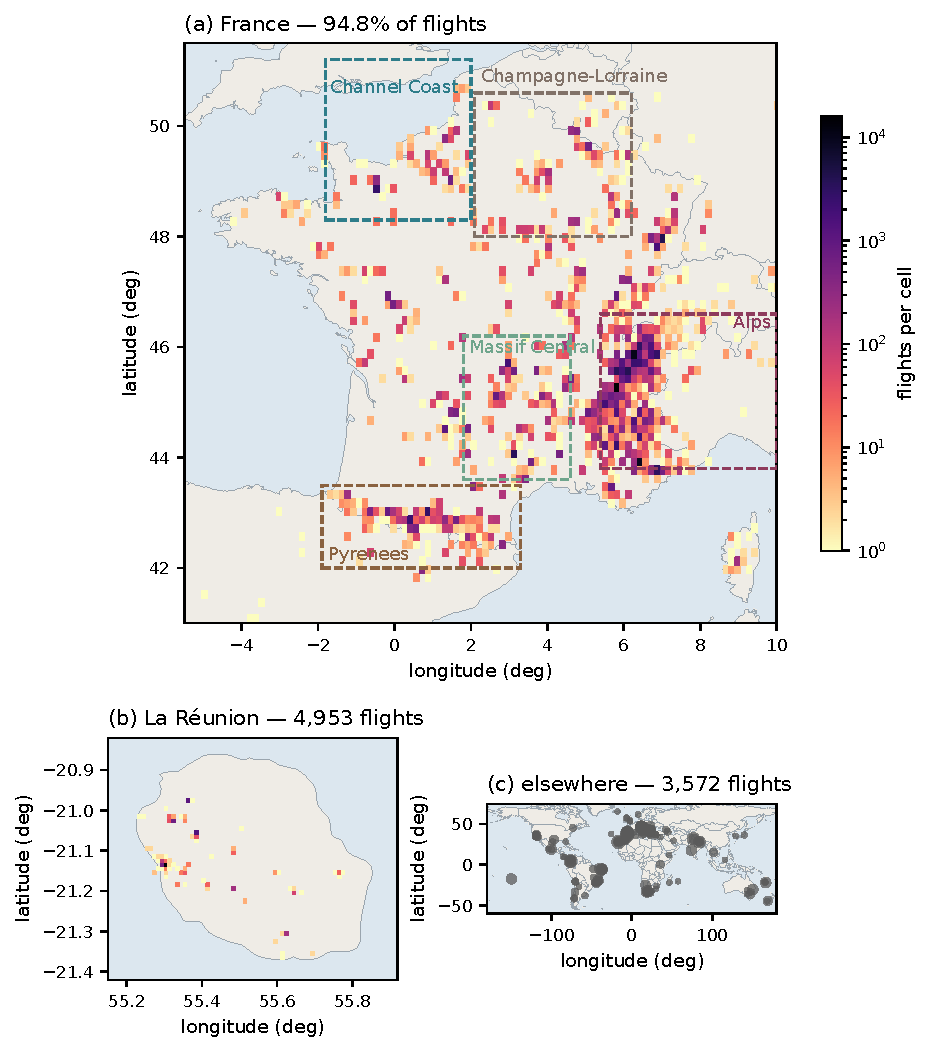
\includegraphics[width=72mm,trim=35bp 176bp 4bp 0bp,clip]{../../thesis/generated/prelim_map.pdf}};
 \txt[text=pisablue,font=\fontsize{12}{14}\selectfont\bfseries]{90}{17}{63}{FFVL distance competition}
 \txt[text=para,font=\fontsize{20}{23}\selectfont\bfseries]{90}{29}{63}{\num{\StatParaDownloaded}}
 \smalltxt[]{90}{38}{63}{Paraglider tracklogs\\1999--2000 to 2025--2026}
 \txt[text=hang,font=\fontsize{20}{23}\selectfont\bfseries]{90}{51}{63}{\num{\StatHangDownloaded}}
 \smalltxt[]{90}{60}{63}{Hang-glider tracklogs\\2001--2002 to 2025--2026}
 \bottomline{IGC trajectories + metadata: time, position, altitude, site, circuit and wing class}
 \credit{Thesis Ch. 2; map: retained flights, both disciplines. Colour = flights per 0.15$^\circ$ cell (log scale).}
\notetext{The source is the FFVL Coupe F\'ed\'erale de Distance, with separate archives for paragliders and hang gliders. The verified downloads contain 186,052 and 6,716 tracklogs. Season names refer to their starting year. The IGC files supply time-stamped coordinates and altitude channels, while the catalogue supplies flight date, declared take-off site, route class and wing class. The map shows the retained population, not the raw downloads; both disciplines are pooled. About 94.8 percent of retained flights are in metropolitan France, with a strong Alpine concentration. Additional flights occur in La R\'eunion and elsewhere. This is a submitted cross-country archive with uneven geographic coverage, not a random sample of all free flight. Sources: thesis Chapter 2; generated/stats.tex, pipeline\_census.tex and prelim\_map.pdf.}
\finishslide\end{frame}

% 4 ------------------------------------------------------------------
\begin{frame}[plain]\frametitle{Cleaning and filtering: the full procedure}\startslide{Cleaning and filtering: the full procedure}
 \foreach \x/\y/\n/\head in {8/18/1/Altitude,58/18/2/Fixes,108/18/3/Airborne interval,8/46/4/Flight selection,58/46/5/Coordinates,108/46/6/Time grid}{
  \fill[pisablight!38](\x,\y)circle(2.8);
  \node[text=pisablue,font=\bfseries\small]at(\x,\y){\n};
  \txt[text=pisablue,font=\bfseries\fontsize{10}{12}\selectfont]{\x+5}{\y-2}{40}{\head}
 }
 \smalltxt[]{8}{24}{43}{GNSS throughout.\\Check presence and range.}
 \smalltxt[]{58}{24}{43}{Remove impossible positions;\\invalidate bad altitudes.}
 \smalltxt[]{108}{24}{43}{Trim ground phases;\\split witnessed ground stops.}
 \draw[->,pisablue](49,30)--(55,30);\draw[->,pisablue](99,30)--(105,30);
 \draw[->,pisablight,line width=.8pt](149,37)--(149,41)--(8,41)--(8,42.5);
 \smalltxt[]{8}{52}{43}{Duration $\geq40$ min\\Path $\geq20$ km; altitude range $\geq600$ m\\Integrity and reach checks}
 \smalltxt[]{58}{52}{43}{Local east and north.\\Keep GNSS altitude.\\One origin per flight.}
 \smalltxt[]{108}{52}{43}{Fill short gaps; split long gaps.\\Flag repairs; smooth\\and differentiate.}
 \draw[->,pisablue](49,60)--(55,60);\draw[->,pisablue](99,60)--(105,60);
 \bottomline{A local outlier flag alone never deletes a fix; impossible steps drive removal}
 \credit{Thesis \S2.7--2.8. Long altitude gaps split the full trajectory as well.}
\notetext{This slide compresses the entire preparation pipeline. GNSS altitude is used end to end; eligible, locally complete barometry is only corroborating evidence for specific cleaning decisions. Horizontal deletion uses physical reachability and a successful return to the trend; the Hampel identifier flags local disagreement but does not gate deletion. Timestamp defects, repeated-position runs and altitude defects have separate rules. Sustained movement defines the outer airborne interval, and sufficiently witnessed interior ground intervals are excised. Flight-level thresholds restrict the population: recorded duration at least 40 minutes, path at least 20 km, altitude range at least 600 m, elapsed span at most 16 hours, plus integrity and reach checks. Coordinates are projected locally, then resampled on the flight's native grid. The gap cap is min(10 times the native cadence, 20 seconds), including gaps between finite altitudes. A Savitzky--Golay step supplies smoothed positions and derivatives. Source: thesis Sections 2.7--2.8 and the two cleaning ADRs.}
\finishslide\end{frame}

% 5 ------------------------------------------------------------------
\begin{frame}[plain]\frametitle{Retain supported motion, record every repair}\startslide{Retain supported motion, record every repair}
 \node[anchor=north west,inner sep=0pt]at(7,16){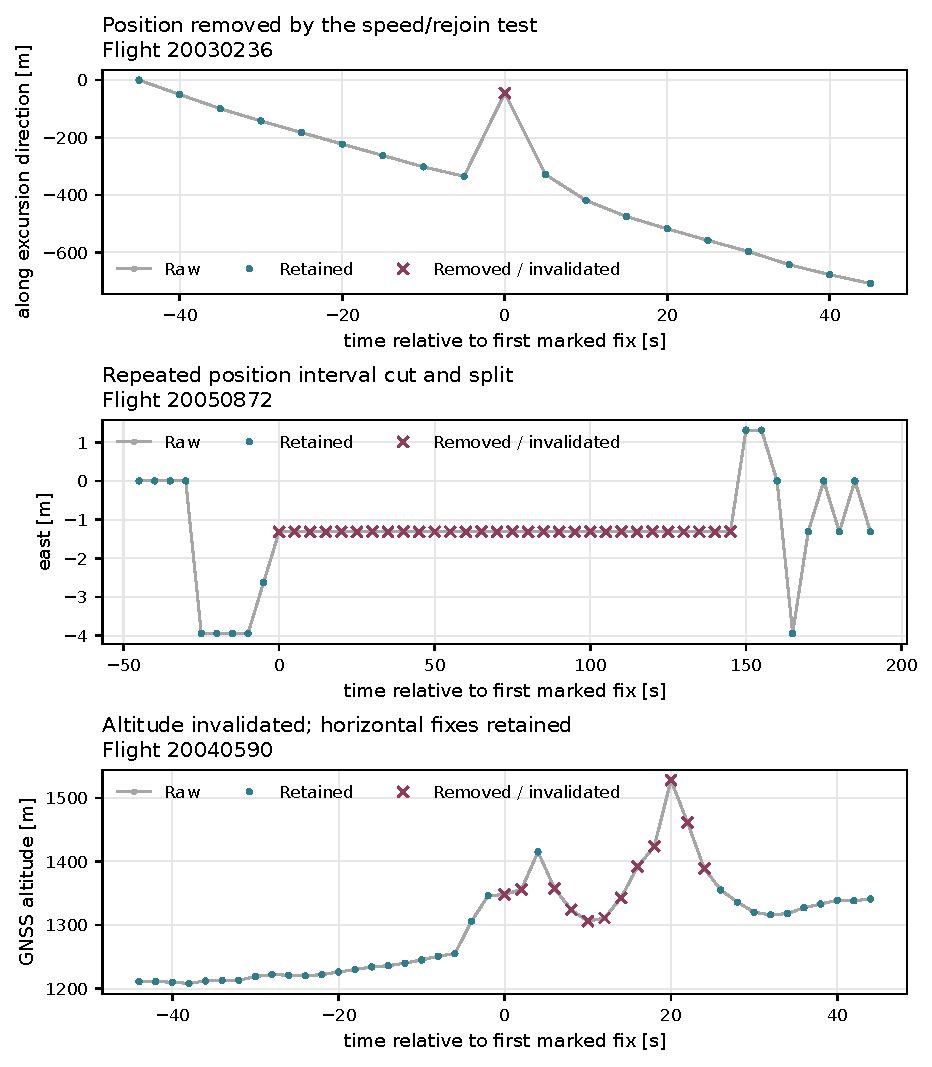
\includegraphics[width=104mm,trim=0bp 338bp 0bp 0bp,clip]{../../thesis/generated/cleaning_real_examples.pdf}};
 \smalltxt[text=pisablue]{116}{22}{36}{Real example:\\remove an impossible excursion when the track rejoins.}
 \smalltxt[]{116}{45}{36}{Long unsupported intervals become boundaries.}
 \draw[pisablight,line width=.6pt](8,59)--(151,59);
 \txt[text=para,font=\fontsize{17}{20}\selectfont\bfseries]{9}{63}{68}{\num{\StatPipeParaKept}\quad\small 84.1\% retained}
 \txt[text=hang,font=\fontsize{17}{20}\selectfont\bfseries]{87}{63}{65}{\num{\StatPipeHangKept}\quad\small 90.7\% retained}
 \smalltxt[text=para]{9}{70}{60}{Paragliders}
 \smalltxt[text=hang]{87}{70}{60}{Hang gliders}
 \bottomline{Paraglider grid reconstruction: 0.58\% \qquad Hang glider: 0.30\%}
 \credit{Thesis \S2.7--2.8; real-example flight 20030236; retention denominator = downloaded tracklogs.}
\notetext{The real example shows a horizontal excursion rejected by the speed/rejoin test, not merely by a local outlier flag. The point of cleaning is to retain supported motion while exposing where information has been removed or reconstructed. It does not certify that every remaining fix is error-free. The full cascade retains 156,406 paraglider flights out of 186,052, and 6,094 hang-glider flights out of 6,716. The percentages on the slide refer to retained flights, whereas 0.58 and 0.30 percent refer to reconstructed grid points within the retained output. These are different denominators. Reconstruction flags are kept, long gaps cause segment boundaries, and transport increments never cross a boundary. These counts describe the cleaned archive; further temporal-resolution and duration restrictions define the samples used below. Sources: generated/cleaning\_real\_examples.pdf and pipeline\_census.tex, thesis Sections 2.7--2.8.}
\finishslide\end{frame}

% 6 ------------------------------------------------------------------
\begin{frame}[plain]\frametitle{Measuring horizontal transport}\startslide{Measuring horizontal transport}
 \draw[para!65,line width=1.5pt] (11,51)..controls(14,43)and(17,39)..(20,42)..controls(30,47)and(35,46)..(43,34)..controls(51,22)and(55,37)..(62,38)..controls(67,40)and(72,40)..(77,33);
 \fill[pisablue](20,42)circle(.9);\fill[pisablue](62,38)circle(.9);
 \draw[-{Latex},pisablue,line width=1pt](20,42)--(62,38);
 \smalltxt[]{13}{48}{30}{$\boldsymbol{x}(t)$}
 \smalltxt[]{56}{43}{33}{$\boldsymbol{x}(t+\tau)$}
 \smalltxt[text=pisablue]{27}{32}{41}{$\Delta\boldsymbol{x}(\tau)$}
 \smalltxt[text=muted]{10}{60}{66}{Displacement is the straight-line change in position, not distance travelled.}
 \txt[]{88}{19}{64}{Average within each flight,\\then give each flight equal weight.}
 \txt[font=\fontsize{12}{16}\selectfont]{87}{36}{67}{$\displaystyle m_f(\tau)=\frac{1}{n_f}\sum_i|\Delta\boldsymbol{x}_{fi}|^2$\\[3mm]$\displaystyle M_2(\tau)=\frac{1}{N}\sum_f m_f(\tau)$}
 \bottomline{$M_2(\tau)\propto\tau^{2H}$:\quad $H=\tfrac12$ diffusion\quad $H=1$ ballistic motion}
 \credit{Thesis \S3.1.1. Within-segment origins only; common 10 s grid for the main analysis.}
\notetext{For each lag, form horizontal displacements between positions within the same retained segment. The displacement is a chord, not the path length. First average squared displacements over every admissible origin in a flight, pooling its selected segments. Then average over flights with equal weight. This prevents long flights from dominating through their number of origins and prevents heavily fragmented flights from gaining weight through their number of segments. For the main analysis, native cadences above ten seconds are excluded and each selected segment is sampled on a common ten-second grid. The 33 physical lags range from ten to ten thousand seconds. A log--log slope is written as 2H; H is an effective growth exponent here, not an established self-similarity parameter of a stochastic process. The standard diffusive and ballistic values are references. Source: thesis Section 3.1.1.}
\finishslide\end{frame}

% 8 ------------------------------------------------------------------
\begin{frame}[plain]\frametitle{Keep the same flights at every lag}\startslide{Keep the same flights at every lag}
 \txt[text=pisablue,font=\bfseries\fontsize{11}{13}\selectfont]{8}{18}{56}{One cohort for 10--10,000 s}
 \txt[]{8}{29}{54}{$\tau_{\max}\leq0.8T_s$\\[2mm]Selected segments last\\at least 12,500 s (3 h 28 min).}
 \txt[text=para,font=\fontsize{16}{19}\selectfont\bfseries]{8}{51}{52}{46,273 paragliders}
 \txt[text=hang,font=\fontsize{14}{17}\selectfont\bfseries]{8}{62}{52}{2,326 hang gliders}
 \figureat{66}{17}{88}{selection}
 \bottomline{Selecting long segments raises $H$ by about 2\% on matched lag ranges}
 \credit{Thesis \S3.1.3. $C_{100}$, $C_{1000}$, $C_{10000}$: fixed cohorts supporting those maximum lags; 90\% intervals.}
\notetext{The available population loses short flights as lag increases. We therefore select a fixed set of flights and segments once, before computing the main curves. Requiring the maximum lag to be at most 80 percent of segment duration leaves at least one fifth of each selected segment available for origins at the longest lag. For ten thousand seconds, that means at least 12,500 seconds on the common grid and at least 251 origins at the maximum lag. Shorter segments of an otherwise eligible flight are excluded at every lag. The main cohort contains 46,273 paragliders and 2,326 hang gliders. The figure compares nested cohorts over identical fit intervals, using paired bootstrap draws. The main cohort increases H by 0.0164--0.0177, about 1.8--2.0 percent. We accept this small, measured duration-selection shift to keep the population constant across three decades of lag. Origins still vary with lag. Source: thesis Section 3.1.3 and ch3\_transport\_report.json.}
\finishslide\end{frame}

% 9 ------------------------------------------------------------------
\begin{frame}[plain]\frametitle{Fast growth persists, but one exponent is a summary}\startslide{Fast growth persists, but one exponent is a summary}
 \figureat{7}{16}{146}{fixed}
 \bottomline{Fixed population: $H_{\rm para}=0.882$\quad $H_{\rm hang}=0.852$\quad over 10--10,000 s}
 \credit{Thesis \S3.1. 1,000 site--day bootstrap draws; pointwise 90\% bands. $H$ is an effective growth exponent.}
\notetext{The fixed-population curves still show growth between the diffusive and ballistic references when summarised over ten to ten thousand seconds. The fitted exponents are 0.882 [0.881,0.883] for paragliders and 0.852 [0.849,0.855] for hang gliders. The local slope changes with lag, so the global fit compresses a curved relationship into a single effective number. Uncertainty is evaluated with one thousand resamples of take-off-site and calendar-day groups, retaining dependence among flights in a group. The same draws are reused over lags and, below, over conditional groups. The bands are pointwise 90 percent intervals, not a simultaneous band for the entire curve. A site--day grouping also does not guarantee independence between all groups; shared weather can remain. These results constrain a model but do not identify a unique stochastic process. Source: thesis Section 3.1 and the fixed-population arrays and fits in ch3\_transport\_report.json.}
\finishslide\end{frame}

% 10 -----------------------------------------------------------------
\begin{frame}[plain]\frametitle{Launch-altitude groups have different MSDs}\startslide{Launch-altitude groups have different MSDs}
 \figureat{6}{17}{104}{altitude}
 \smalltxt[text=pisablue,font=\fontsize{9}{11}\selectfont\bfseries]{115}{18}{39}{Initial GNSS altitude}
 \smalltxt[]{115}{28}{39}{Plains: $<300$ m\\[1mm]Hills: 300--800 m\\[1mm]Low mountains:\\800--1,500 m\\[1mm]High mountains:\\$\geq1,500$ m}
 \smalltxt[text=muted]{115}{58}{39}{Above sea level, at the first cleaned fix.}
 \bottomline{Pooled lowland curves grow faster; circuit composition also changes with altitude}
 \credit{Thesis \S3.2.1. Paragliders, fixed cohort; altitude is a launch-environment proxy, not measured relief.}
\notetext{The four groups partition the fixed paraglider cohort by GNSS altitude at the first cleaned fix. Altitude is measured above sea level. The conventional labels are Plains, Hills, Low mountains and High mountains; they do not measure local slope or terrain along the route. Their sizes are 1,844, 2,908, 22,097 and 19,424. The effective exponents are approximately 0.950, 0.929, 0.866 and 0.875. The high-mountain exponent is slightly larger than the low-mountain one, so even the pooled ordering is not monotonic in altitude. Circuit composition is very different: the open-route shares are 91.1 and 71.1 percent in the two lowland groups, compared with 33.5 and 35.0 percent in the mountain groups. Consequently the pooled difference is an association, not an isolated effect of orography. We resolve the circuit dependence on slide 13. Source: thesis Section 3.2.1 and ch3\_conditional.json.}
\finishslide\end{frame}

% 11 -----------------------------------------------------------------
\begin{frame}[plain]\frametitle{Region matters within a broad launch environment}\startslide{Region matters within a broad launch environment}
 \figureat{7}{16}{146}{regions}
 \bottomline{Alps--Pyrenees: $\Delta H=0.037$\qquad Lowland pair: $\Delta H=-0.002$, interval includes zero}
 \credit{Thesis \S3.2.1. Geographic boxes crossed with initial altitude; circuits and equipment pooled.}
\notetext{This comparison holds the broad altitude setting fixed within geographic boxes. The Alpine and Pyrenean groups retain only launches at or above 800 metres; the two lowland groups retain only launches below 800 metres. There are 32,790 Alpine flights, 2,257 Pyrenean flights, 1,068 Channel Coast flights and 798 Champagne-Lorraine flights. Alpine H is 0.870 versus 0.833 in the Pyrenees; their paired difference is 0.037 [0.033,0.041]. The lowland exponents are 0.953 and 0.955, with difference -0.002 [-0.005,0.001]. A similar exponent does not imply identical motion: displacement amplitudes and curve shapes can differ. These selections do not match weather, route composition, exact altitude, site or equipment. The regional contrast is descriptive and does not identify the effect of mountain geometry or thermal triggers. Source: thesis Section 3.2.1; ch3\_conditional.json.}
\finishslide\end{frame}

% Thermal viewer ------------------------------------------------------
\begin{frame}[plain]\frametitle{Thermal patterns across height}\startslide{Thermal patterns across height}
 \smalltxt[]{7}{16}{146}{Viewer: intersect climb-labelled trajectories with horizontal planes.}
 \smalltxt[text=muted]{7}{21}{146}{Within each cell: same dates, segmentation and map bounds at both heights.}
 \txt[align=center,text=pisablue,font=\bfseries\fontsize{11}{13}\selectfont]{7}{27}{71}{Mountains}
 \txt[align=center,text=pisablue,font=\bfseries\fontsize{11}{13}\selectfont]{82}{27}{71}{Plains}
 \foreach \xx/\zz in {7/\ThermalLower,44.5/\ThermalUpper,82/\ThermalLower,119.5/\ThermalUpper}{
  \smalltxt[align=center]{\xx}{33}{33.5}{$z_{\mathrm{AGL}}=\zz$}
 }
 \thermalpanel{7}{38}{mountain-low}{Mountain cell\\lower plane}
 \thermalpanel{44.5}{38}{mountain-high}{Mountain cell\\higher plane}
 \thermalpanel{82}{38}{plains-low}{Plains cell\\lower plane}
 \thermalpanel{119.5}{38}{plains-high}{Plains cell\\higher plane}
 \fill[pisablight!33](7,74.7)rectangle(153,83);
 \smalltxt[text=pisablue,font=\fontsize{9}{11}\selectfont]{10}{75.5}{140}{Working observation: mountain patterns shift less with height than lowland patterns.}
 \smalltxt[text=pisablue,font=\fontsize{8}{10}\selectfont]{10}{79.6}{140}{Possible explanations: stronger uplift or weaker wind; neither is measured here.}
 \credit{Dots are climb crossings, not thermal centres. $z_{\mathrm{AGL}}$ is relative to a fixed reference for each cell.}
\notetext{The viewer lets us inspect the spatial pattern of observed climb crossings at different horizontal planes. We compare the same mountain cell at two heights and the same plains cell at those heights, keeping the selected dates, segmentation method and map bounds fixed within each pair. The qualitative observation is that the mountain pattern appears more vertically aligned, whereas the lowland pattern shifts more as the plane rises. This concerns horizontal position as a function of height, not stationarity in time and not a change in the vertical coordinate of a fixed plane. Stronger uplift could shorten the time available for horizontal advection over a given height increment; weaker horizontal wind could also reduce that displacement. Terrain-anchored lift is another possible contributor. These are hypotheses, not causes established by these views. The dots are observed climb crossings, possibly several per thermal, not identified thermal centres or independent thermals. Different flights can support the two heights. In this viewer, AGL is height above a fixed cell reference derived from starting altitudes, not pointwise height above a terrain model. Source: docs/guide/thermal-planes.md; qualitative interpretation proposed by the presenter.}
\finishslide\end{frame}

% 12 -----------------------------------------------------------------
\begin{frame}[plain]\frametitle{Open routes have larger displacement growth}\startslide{Open routes have larger displacement growth}
 \figureat{6}{17}{104}{circuit}
 \smalltxt[text=para,font=\bfseries\fontsize{10}{12}\selectfont]{116}{19}{36}{Open circuits}
 \draw[para,line width=1.2pt,-{Latex}](117,36)--(127,31)--(133,34)--(149,27);
 \smalltxt[]{116}{39}{36}{17,961 flights}
 \smalltxt[text=wine,font=\bfseries\fontsize{10}{12}\selectfont]{116}{50}{36}{Closed circuits}
 \draw[wine,line width=1.2pt,-{Latex}](117,66)--(132,57)--(149,67)--(117,66);
 \smalltxt[]{116}{69}{36}{28,234 flights}
 \bottomline{$H_{\rm open}-H_{\rm closed}=0.054\;[0.053,\,0.056]$\quad (90\% paired interval)}
 \credit{Thesis \S3.2.2. Catalogue declarations; 78 unclassified flights excluded. Route drawings are schematic.}
\notetext{The catalogue describes the intended circuit, not a guarantee that the recorded trimmed trajectory returns to its starting point. Closed routes include triangles and out-and-return flights. Pooling launch altitudes gives H=0.910 for open routes and 0.856 for closed routes. Their paired difference is clearly positive under the adopted bootstrap. Turning back can reduce net displacement over intervals spanning a turn. However, lag is averaged over origins throughout a segment: there is no universal onset at half or one third of flight duration, and ten thousand seconds is an analysis limit, not a shared total duration. The route schematics illustrate geometry only. The pooled comparison still mixes launch environments and other conditions, so its magnitude cannot rank the causal importance of route choice against terrain. Sources: thesis Section 3.2.2, ch3\_conditional.json.}
\finishslide\end{frame}

% 13 -----------------------------------------------------------------
\begin{frame}[plain]\frametitle{The altitude ordering reverses for closed routes}\startslide{The altitude ordering reverses for closed routes}
 \figureat{7}{16}{146}{interaction}
 \bottomline{Open: lowland $H$ is higher \qquad\qquad Closed: mountain $H$ is higher}
 \credit{Thesis \S3.2.2. Same 10--10,000 s fits; 90\% paired-bootstrap intervals. Connecting lines guide the eye.}
\notetext{This is the key joint comparison. The plotted points are fitted exponents from the same four altitude classes, separated into open and closed circuits. For open routes, the lowland-minus-mountain contrasts are positive, between 0.051 and 0.064. For closed routes, they are negative, with magnitudes between 0.021 and 0.051. All eight paired intervals exclude zero. Open routes also have larger H than closed routes within each altitude class. The smallest cell is 165 closed flights in Plains, so its uncertainty is visibly larger. The observed altitude association changes sign with circuit type; a universal claim that mountain launch environments suppress transport growth is therefore not supported. Possible mechanisms include the organisation of lift, detours and differences in circuit size or turn times, but these are hypotheses. The figure establishes conditional orderings, not their causal explanation. Source: thesis Section 3.2.2; ch3\_conditional.json and ch3\_transport\_task\_table.tex.}
\finishslide\end{frame}

% 14 -----------------------------------------------------------------
\begin{frame}[plain]\frametitle{The equipment contrast survives altitude stratification}\startslide{The equipment contrast survives altitude stratification}
 \figureat{7}{16}{146}{equipment}
 \bottomline{Higher $H$ for EN D/CCC in every altitude class; largest gap in Low mountains}
 \credit{Thesis \S3.2.3. Wing class is an equipment and experience proxy, not a measured pilot-skill category.}
\notetext{The two equipment groups contain 27,609 flights on EN A/B/C wings and 16,497 on EN D/CCC wings; 2,167 flights are excluded from this comparison. The thesis calls them beginners and experts as an operational proxy. Individual experience is not observed: an experienced pilot can fly a lower-class wing, and the same pilot can contribute to different groups on different flights. The pooled exponent difference is 0.025 [0.024,0.026]. Within altitude classes the differences are 0.013, 0.013, 0.021 and 0.016, all with paired intervals excluding zero. The Low mountains contrast exceeds the others in the paired interaction tests. A constant speed multiplier alone changes MSD amplitude, not its log--log slope, so the difference concerns the lag dependence too. It still mixes wing performance, pilots, routes and conditions. Source: thesis Section 3.2.3, ch3\_conditional.json and ch3\_conditional\_equipment\_table.tex.}
\finishslide\end{frame}

% 15 -----------------------------------------------------------------
\begin{frame}[plain]\frametitle{What the measurements establish}\startslide{What the measurements establish}
 \txt[text=pisablue,font=\bfseries\fontsize{15}{18}\selectfont]{9}{19}{11}{01}
 \txt[]{25}{19}{126}{Rapid horizontal spreading in both disciplines,\\with an effective exponent that changes across scales.}
 \draw[pisablight](25,34)--(151,34);
 \txt[text=pisablue,font=\bfseries\fontsize{15}{18}\selectfont]{9}{40}{11}{02}
 \txt[]{25}{39}{126}{The altitude association depends on the declared circuit:\\the lowland--mountain ordering reverses for closed routes.}
 \draw[pisablight](25,54)--(151,54);
 \txt[text=pisablue,font=\bfseries\fontsize{15}{18}\selectfont]{9}{60}{11}{03}
 \txt[]{25}{59}{126}{Equipment-group differences remain within altitude classes;\\their physical and behavioural contributions are still mixed.}
 \bottomline{Next: explain global transport through flight behaviour and physical models}
 \credit{Results through thesis \S3.2. Conditional findings describe the fixed cohort of long paraglider flights.}
\notetext{The work so far delivers a traceable dataset and a set of empirical constraints for transport modelling. Both disciplines show rapid displacement growth, but a single effective exponent is not the whole story. Keeping flights and segments fixed separates lag dependence from changing membership. Among long paraglider flights, launch environment, region, route and equipment all carry structure. Most notably, the altitude ordering reverses between open and closed routes, and the equipment contrast persists within altitude classes. These are observed associations, not isolated causal effects. The next stage is to connect the global results to flight behaviour and test physical stochastic models against several observables under the same measurement protocol. The thermal-plane view adds a qualitative observation about vertical alignment. It does not establish a quantitative thermal-displacement law or identify its mechanism. Sources: current thesis introduction and Sections 3.1--3.2; thermal-plane viewer documentation.}
\finishslide\end{frame}

\end{document}
